\documentclass{article}
    
\usepackage{Haust2017skil}
\usepackage{caption}
\usepackage{subcaption}

\title{Stærðfræðimynstur í tölvunarfræði \\ Skilaverkefni 12}
\author{}

\begin{document}
\maketitle

Skila skal þessu verkefni á vefnum \href{https://gradescope.com/courses/9487}{Gradescope}. Aðgangskóði fyrir námskeiðið er \textbf{9N834D}.
Þeim má skila sem einstaklingar eða \emph{tvö og tvö saman}.

Gradescope tekur við .pdf skjölum. Frágangur á þeim skiptir máli. Þau skulu vera hreinskrifuð í tölvu. 
%Kerfi eins og \LaTeX, Google Docs og Microsoft Word geta búið til .pdf skjöl. 
Mikilvægt er að merkja á hvaða blaðsíðu .pdf skjalsins hver lausn kemur fyrir, ekki er hægt að gera ráð fyrir að dæmatímakennarar fari yfir ómerkt dæmi.

Telji nemandi að mistök hafi verið gerð við yfirferð skal tilkynna slíkt með tölvupósti til dæmatímakennara. Nálgast má lista yfir hvaða dæmatímakennari fór yfir hvaða dæmi á Piazza-vef námskeiðsins.

\section{Kaflar 10 og 11}

\question 


\paragraph{(Ísl)} Öll tré með a.m.k. tvo hnúta eru tvíhlutanet. Rökstyðjið.

\paragraph{(En)} Every tree with two or more vertices is bipartite. Explain why.

\paragraph{Í bók:} Þetta dæmi er ekki í bókinni.


\section{Kafli 10.7}

\question Eru eftirfarandi net lagnet? Sé svo, teiknið tilsvarandi sléttunet. Sé svo ekki, gefið ástæðu.

\begin{center}
    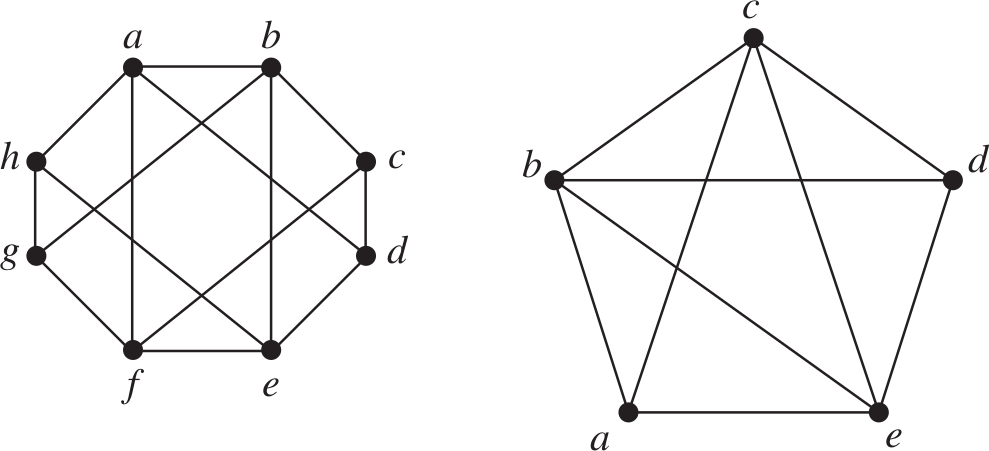
\includegraphics[width=0.5\textwidth]{graph-maybe-planar}
\end{center}

\paragraph{Í bók:} Byggt á fyrstu æfingum í kafla 10.7.

\question

Lítum á lagnet sem hefur $k$ samhengisþætti, $e$ leggi og $v$ hnúta. Sléttunet lagnetsins skiptir sléttunni í $r$ möskva.

Finnið formúlu fyrir $r$ út frá $e$, $v$ og $k$.

\paragraph{Í bók:} 10.7.18 í International/Icelandic, 10.7.14 í Global

\section{Kafli 10.8}

\question Fjarlægðir á milli sex útvarpssendistöðva í kílómetrum eru gefnar á eftirfarandi töflu.

\begin{center}

\begin{tabular}{ccccccc}
\toprule
&1&2&3&4&5&6\\
\midrule
1&-&85&175&200&50&100\\
2&85&-&125&175&100&160\\
3&175&125&-&100&200&250\\
4&200&175&100&-&210&220\\
5&50&100&200&210&-&100\\
6&100&160&250&220&100&-\\
\bottomrule
\end{tabular}

\end{center}
Hversu margar mismunandi útvarprásir þurfa þessar stöðvar, ef tvær stöðvar geta ekki notað sömu rásina séu þær innan 150 kílómetra hver frá annarri?

Leysið verkefnið með því að setja fram net og ákvarða fyrir það litunartölu.

\paragraph{Í bók:} Exercise 10.8.18 í International/Icelandic, 10.8.12 í Global

\section{Kafli 11.1}

\question Keðjubréf nokkurt byrjar þegar manneskja sendir bréfið á fimm aðrar manneskjur. Allir sem fá bréfið senda það annaðhvort til fimm annarra sem ekki hafa fengið bréfið áður eða senda það ekki áfram á neinn.

Gefum okkur að 10000 manneskjur sendi bréfið áður en það fjaraði út og að enginn fái bréfið tvisvar. Hversu margir fengu bréfið og hve margir sendu það ekki áfram? Útskýrið með hugtökum sem tengjast trjám.

\paragraph{Í bók:} Exercise 11.1.22 í International/Icelandic, 11.1.16 í Global

\section{Kafli 11.3}

\question 

Í hvaða röð eru hnútar trésins heimsóttir með trjáflakki í miðröð?

\begin{center}
    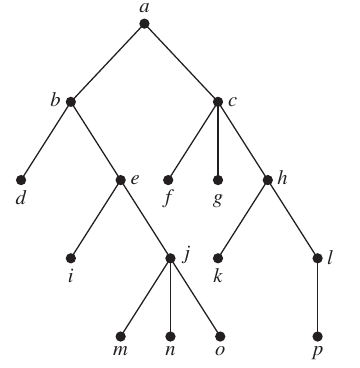
\includegraphics[width=0.5\textwidth]{tree-to-traverse}
\end{center}

\paragraph{Í bók:} Exercise 11.3.11 í International/Icelandic, 11.3.6 í Global

\end{document}
